%!TEX root = sdm-2018.tex
\appendix

\section{Proofs}

\subsection{}
The following lemma states that the information retrieved via
\parentstransitions\ monitoring operations decrease the expected uncertainty
about the positioning of items after the transition step.

\begin{lemma}
\[
\objective_{_\shortparentstransitions}(S) \leq \uncertainty_0
\]
\label{lemma:decreased_uncertainty_pt}
\end{lemma}
\begin{proof}
Indeed, using Equations~\eqref{eq:adjustedx} and~\eqref{eq:adjustedP} to expand 
Equation~\eqref{eq:nodevariance} we have
\begin{align}
\objective_{_\shortparentstransitions}(S) =\ & \sum_{u\in V}\initial^{\prime}(u)\sum_{v\in V\setminus S}\transition^{\prime}(u,v)\left(1-\transition^{\prime}(u,v)\right) \nonumber \\
  =\ & \sum_{u\in V}\initial(u)\sum_{v\in V\setminus S}\transition(u,v)\left(1-\frac{\transition(u,v)}{1-\rho(u,S)}\right) \nonumber  \\
  \leq\ & \sum_{u\in V}\initial(u)\sum_{v\in V\setminus S}\transition(u,v)\left(1-\transition(u,v)\right) \nonumber \\
  =\ & \objective_{_\shortparentstransitions}(\emptyset). \nonumber
\end{align}
\end{proof}


\subsection{}
The following theorem states that, for the same set of monitored nodes,
\parentstransitions\ and \nodeitems\ lead to the same value of the objective 
function.
\begin{theorem}
\label{theorem:node-equivalence}
$\objective_{_\shortnodeitems}(S) = \objective_{_\shortparentstransitions}(S)$
\begin{proof}
We express $\uncertainty(A_{_\shortnodeitems})$ in terms
of $\uncertainty(A_{_\shortparentstransitions})$ as follows.
(We write `c.w.' for `consistent with').
\begin{align}
\uncertainty(A_{_\shortnodeitems})
 = \sum_{A_{_\shortparentstransitions}
  \ \text{c.w.}\; A_{_\shortnodeitems}
  } \uncertainty(A_{_\shortparentstransitions})
  \prob(A_{_\shortparentstransitions} | A_{_\shortnodeitems})
\end{align}


We can now use the above equation to
express the expected uncertainty $\objective_{_\shortnodeitems}(S)$
in terms of $\objective_{_\shortparentstransitions}(S)$ as:
\begin{align}
\objective_{_\shortnodeitems}(S) & =  E[\uncertainty(A_{\shortnodeitems})] \nonumber \\
& = \sum_{A_{_\shortnodeitems}}\uncertainty(A_{\shortnodeitems}) \prob(A_{_\shortnodeitems}) = \nonumber \\
& = \sum_{A_{_\shortnodeitems}}\;\;\sum_{A_{_\shortparentstransitions}
  \ \text{c.w.}\ A_{_\shortnodeitems}
  } \uncertainty(A_{_\shortparentstransitions})
  \prob(A_{_\shortparentstransitions} | A_{_\shortnodeitems}) \prob(A_{_\shortnodeitems}) \nonumber \\
& = \sum_{A_{_\shortnodeitems}}\;\;\sum_{A_{_\shortparentstransitions}
  \ \text{c.w.}\ A_{_\shortnodeitems}
  } \uncertainty(A_{_\shortparentstransitions})
  \prob(A_{_\shortparentstransitions}, A_{_\shortnodeitems}) \nonumber \\
& = \sum_{A_{_\shortnodeitems}}\;\;\sum_{A_{_\shortparentstransitions}
  \ \text{c.w.}\ A_{_\shortnodeitems}
  } \uncertainty(A_{_\shortparentstransitions})
  \prob(A_{_\shortparentstransitions}) \nonumber \\
& = \sum_{A_{_\shortparentstransitions}} 
  \uncertainty(A_{_\shortparentstransitions})
  \cdot \prob(A_{_\shortparentstransitions}) \nonumber \\
& = \objective_{_\shortparentstransitions}(S),
\end{align}
which concludes the proof.
\end{proof}
\end{theorem}


\subsection{}

The following lemma states that, with choice restricted 
among the outgoing edges of a node, the optimal
objective value in the \edgetransitions\ setting is obtained for
the edges of highest transition probability.
\begin{lemma}
\begin{equation}
ISOL_i(m) =  \objective_i(D_i^m)	
\end{equation}
\begin{proof}
The optimization function is proportional to the following quantity:
\begin{equation}
f(E) \propto (\sum_{i\in D_u(E)} p_i) - {\sum_{i\in D_u(E)} p_i^2} / {(\sum_{i\in D_u(E)} p_i)}
\end{equation}
where $D_u(E)$ are the remaining (i.e., non-queried) outgoing edges of
parent-node $u$.

Consider two sets of edges $E_0$, $E_1$ $\subseteq O(u)$ of the same size,
all outgoing from a
single parent-node $u$, that differ only at one element.
The probabilities of the corresponding sets of {\bf remaining} edges
are:
\begin{equation}
 D_u(E_0): \{p_0\} \cup C;\;\;\;\;D_u(E_1): \{p_1\} \cup C
\end{equation}
where $p_0, p_1\not\in C$, $p_0 \leq p_1$.

Let $S = \sum_{i\in C} p_i$ and $SS = \sum_{i\in C} p_i^2$.
We take the difference of the optimization functions for the two sets $E_0$
and $E_1$.
\begin{align*}
	f(E_0) - f(E_1) \propto\ & p_0 - p_1 -  \frac{\sum_{i\in D_u(E_0)}{p_i^2}}{\sum_{i\in D_u(E_0)}{p_i}}  
		+  \frac{\sum_{i\in D_u(E_1)}{p_i^2}}{\sum_{i\in D_u(E_1)} {p_i}} \\
	& = - (p_1 - p_0)\frac{SS + S^2}{(S + p_0)(S + p_1)} \leq 0.
\end{align*}
The above shows that selecting the set of edges so that the remaining edges
are associated with smaller probabilities leads to lower (better) values of the
optimization function.
\end{proof}
\label{lemma:singlenodeoptimality}
\end{lemma}

\subsection{}
The following theorem concerns the optimality of algorithm \edgeDP.
\begin{theorem}
\edgeDP\ is optimal for the \edgetransitions\ variant of 
the \mcproblem\ problem.
\label{theorem:edgeDP}
\end{theorem}
\begin{proof}
The proof follows from Lemma~\ref{lemma:singlenodeoptimality}
and by construction of the dynamic programming algorithm
(Equation~\eqref{eq:dptop}).
\end{proof}

\section{Additional Results}
\label{sec:additional_results}
%\subsection{Performance of greedy algorithms on {\geo} graphs.}
Figure~\ref{fig:geo_nodes}
shows the performance of the {\nodegreedy} algorithm for the 
the {\geo} graphs, with each plot corresponding to a different item
distribution schemes.
Observe that {\nodegreedy} significantly outperforms
all other baselines, which capture different semantics of centrality.
In particular, we observe that {\nodegreedy} achieves zero or near-zero
expected uncertainty with a small fraction of selected nodes compared to baselines.
Among the baselines, {\closeness} performs second-best in many cases,
while {\indegree} performs as well as {\closeness} for small $k$.

Similarly, Figure~\ref{fig:geo_edges} shows the 
performance of the different algorithms for the {\edgeproblem} and the {\geo} 
graphs, for all
possible item-distribution schemes.
As before, we observe that {\edgegreedy} outperforms the baselines in all 
cases. We notice also that the pattern of performance differs somewhat for the 
case of {\ego} item distribution. With the exception of one 
baseline ({\probability}), all algorithms achieve steep decline in expected uncertainty for
small value of $k$ - {\edgegreedy} performs best, but baselines are competitive. 
However, for larger $k$, the performance of baselines  
does not keep up with that of {\edgegreedy}.
We believe that this is can be explained as follows:
the first edges selected by 
baselines are either central in terms of graph structure 
-- and therefore near the part of the graph with high concentration of items 
({\edgebetweenness}) -- or directly in the area of the graph with many items 
({\edgenumitems}). 
In terms of reducing expected uncertainty, this is beneficial at first. However, these baselines
as they do not optimize our objective are not able to continue reducing the expected
uncertainty with their subsequent selections.

Figure~\ref{fig:ass_nodes} and Figure~\ref{fig:ass_edges} show the performance of 
the greedy algorithms on the {\nodeproblem} and the {\edgeproblem} problems
respectively. We observe that both the {\nodegreedy} and the {\edgegreedy} algorithms
are consistently the best when compared to the baselines. However, $k=50$ represents
about 1\% of the total edges in the graph, hence their monitoring does not decrease
the uncertainty significantly.
While experiments with larger values of $k$ are prohibitive due to time complexity of the {\edgegreedy} algorithm, we postulate that the greedy algorithm will still continue
outperforming the baselines.

Figures~\ref{fig:ba3_nodes} and ~\ref{fig:ba3_edges} provide a similar comparison
for the different configurations of the {\ba} graph. The greedy algorithms
provide marginal benefits or perform on par with competitive baselines. On the
{\ba} graphs, for {\direct}, {\uniform} and {\inverse} item distributions, some baselines
perform exactly the same as the greedy algorithms for relatively small number of
monitoring operations i.e., $k=50$. Lastly, we observe similar trends in case of the
{\grid} graphs as evident in Figures~\ref{fig:grid_nodes} and ~\ref{fig:grid_edges}.
It should be noted that there is no baseline method that provides a consistently competitive
performance with the greedy algorithms across all different configurations described above.
\balance

\begin{figure*}
\centering
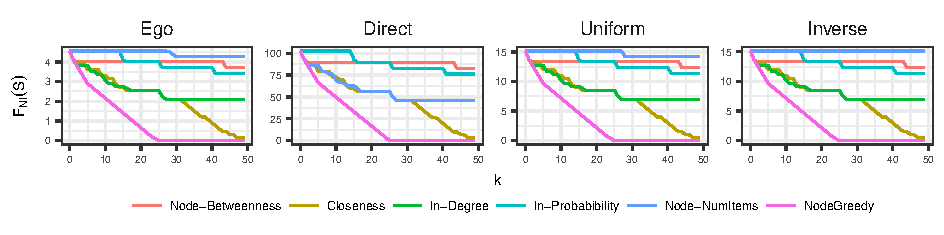
\includegraphics{figures/geo_nodes.pdf}
\caption{{\nodeproblem} {\geo} dataset; $y$-axis expected uncertainty, 
$x$-axis: number of monitored nodes ($k$).}
\label{fig:geo_nodes}
\end{figure*}

\begin{figure*}
\centering
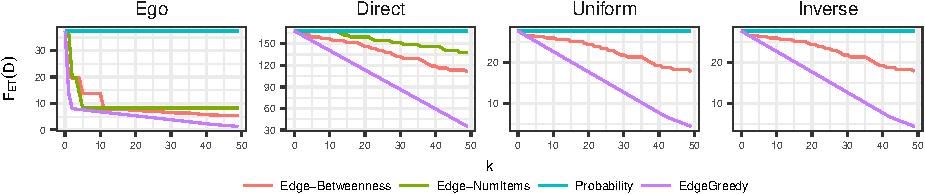
\includegraphics{figures/geo_edges.pdf}
\caption{{\edgeproblem} {\geo} dataset; $y$-axis expected uncertainty, 
$x$-axis: number of monitored edges ($k$).}
\label{fig:geo_edges}
\end{figure*}

\begin{figure*}
\centering
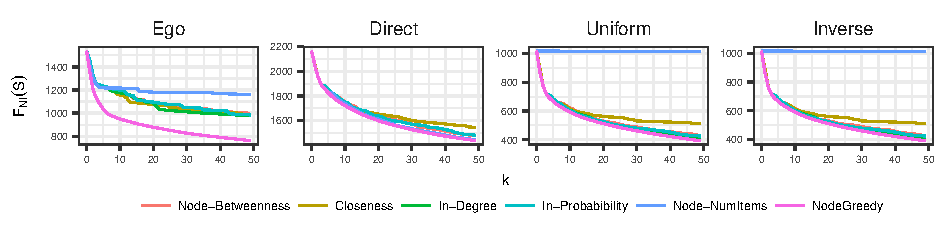
\includegraphics{figures/ass_nodes.pdf}
\caption{{\nodeproblem} {\autonomoussystems} dataset; $y$-axis expected uncertainty, 
$x$-axis: number of monitored nodes ($k$).}
\label{fig:ass_nodes}
\end{figure*}

\begin{figure*}
\centering
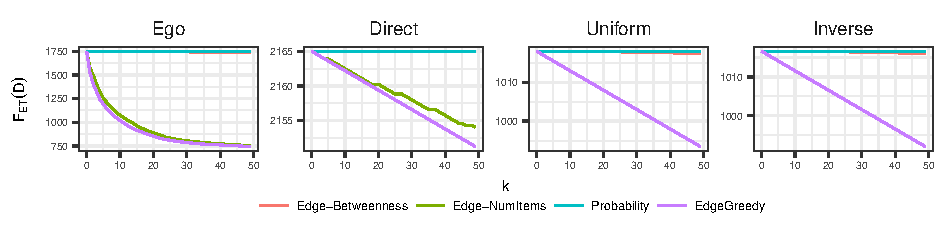
\includegraphics{figures/ass_edges.pdf}
\caption{{\edgeproblem} {\autonomoussystems} dataset; $y$-axis expected uncertainty, 
$x$-axis: number of monitored edges ($k$).}
\label{fig:ass_edges}
\end{figure*}

\begin{figure*}
\centering
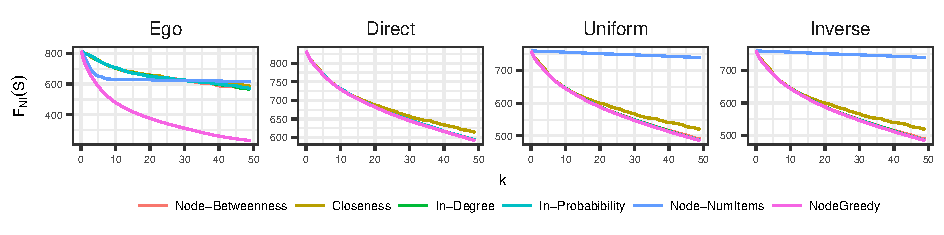
\includegraphics{figures/ba3_nodes.pdf}
\caption{{\nodeproblem} {\ba} dataset; $y$-axis expected uncertainty, 
$x$-axis: number of monitored nodes ($k$).}
\label{fig:ba3_nodes}
\end{figure*}

\begin{figure*}
\centering
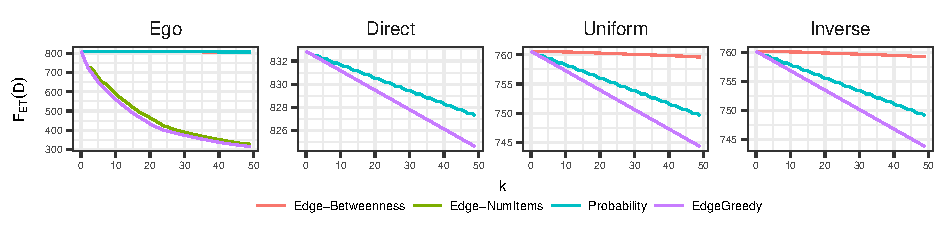
\includegraphics{figures/ba3_edges.pdf}
\caption{{\edgeproblem} {\ba} dataset; $y$-axis expected uncertainty, 
$x$-axis: number of monitored edges ($k$).}
\label{fig:ba3_edges}
\end{figure*}

\begin{figure*}
\centering
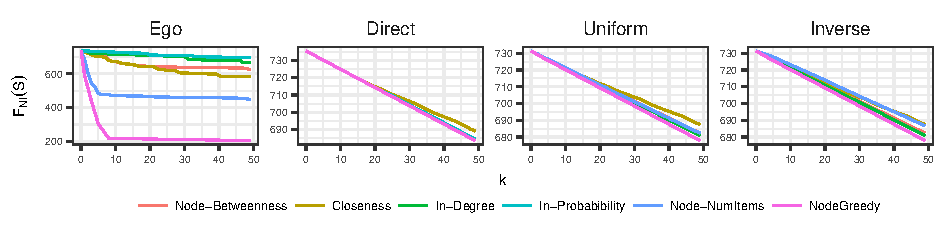
\includegraphics{figures/grid_nodes.pdf}
\caption{{\nodeproblem} {\grid} dataset; $y$-axis expected uncertainty, 
$x$-axis: number of monitored nodes ($k$).}
\label{fig:grid_nodes}
\end{figure*}

\begin{figure*}
\centering
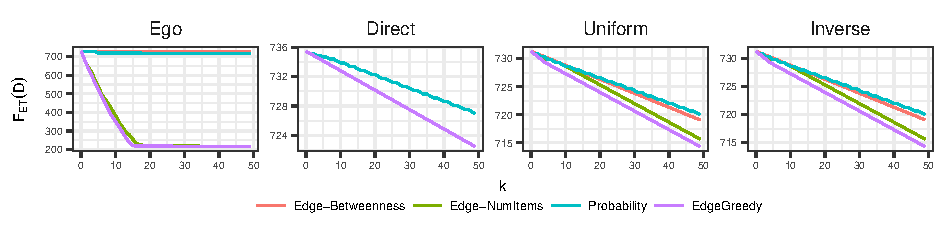
\includegraphics{figures/grid_edges.pdf}
\caption{{\edgeproblem} {\grid} dataset; $y$-axis expected uncertainty, 
$x$-axis: number of monitored edges ($k$).}
\label{fig:grid_edges}
\end{figure*}